\section{Results}

\subsection{1-D model}

\begin{figure}[here]
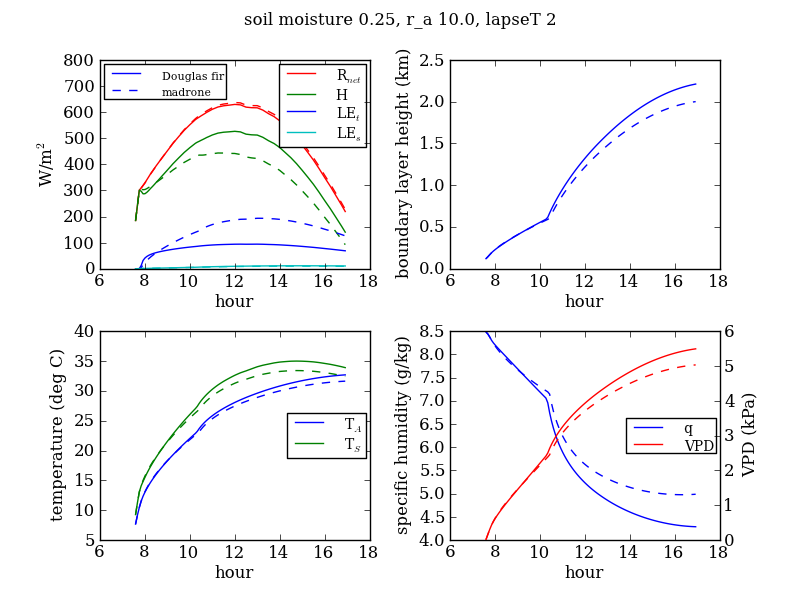
\includegraphics[width=1\textwidth]{ch2-BL/figures/testall_Aug15_soilm0pt25_ra10_lapseT2.png}
\caption{}
\label{fig:BL_1Ddiurnal}
\end{figure}

The 1-D model simulates a reasonable diurnal cycle, but with temperatures several degrees higher than observations.  Figure \ref{fig:BL_1Ddiurnal} shows a typical diurnal cycle for a moderate lapse rate (\#2) and relative soil moisture ($\theta_{rel}$) $= 0.25$.  The Pacific madrone forest has higher transpiration than the Douglas fir forest, because Pacific madrone stomatal conductance is higher at this value of $\theta_{rel}$ (c.f. Figure XX); both cases have very little soil evaporation at this value of $\theta_{rel}$.  As a result, the Pacific madrone case has lower sensible heat ($H$) than the Douglas fir case, leading to a shallower, cooler, and moister boundary layer over the Pacific madrone forest.

\begin{figure}[here]
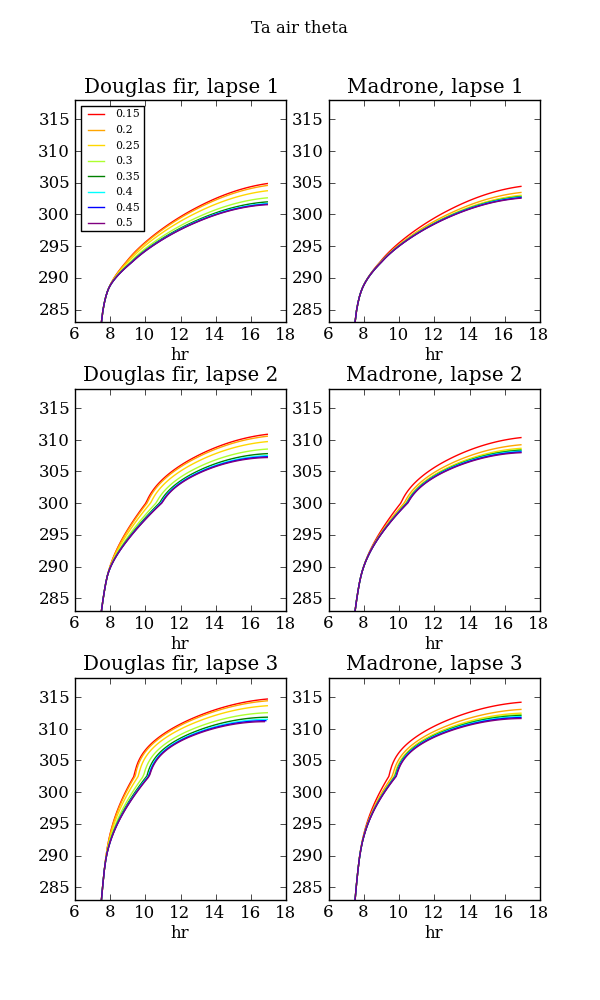
\includegraphics[width=0.5\textwidth]{ch2-BL/figures/testall_compare_sm_lapse_Ta.png}
\caption{}
\label{fig:BL_1DdiurnalTa}
\end{figure}

\begin{figure}[here]
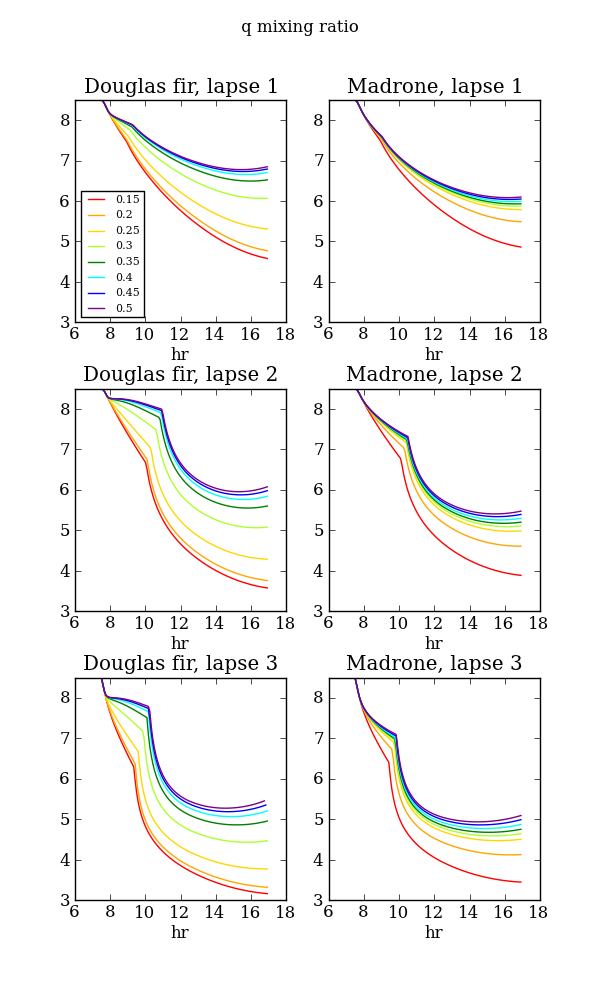
\includegraphics[width=0.5\textwidth]{ch2-BL/figures/testall_compare_sm_lapse_q.png}
\caption{}
\label{fig:BL_1DdiurnalQ}
\end{figure}

%\clearpage

The boundary layer is warmer and drier when the free troposphere is warmer and drier (Figures \ref{fig:BL_1DdiurnalTa} and \ref{fig:BL_1DdiurnalQ}; increasing $T_a$ and decreasing $Q$ from lapse rate 1 to 2 to 3).  Additionally, the shape of the diurnal cycle differs among the free troposphere cases, with most rapid morning increase in $T_a$ in the hottest case (lapse rate 3), due to entrainment of high-$\Theta$ air in the steep low-level inversion.  The drier free troposphere conditions in lapse rate 3 also leads to lower $Q$, but with a slower morning decline of $Q$ because of relatively slow boundary layer growth through the steep inversion.

\begin{figure}[here]
\begin{subfigure}{0.5\textwidth}
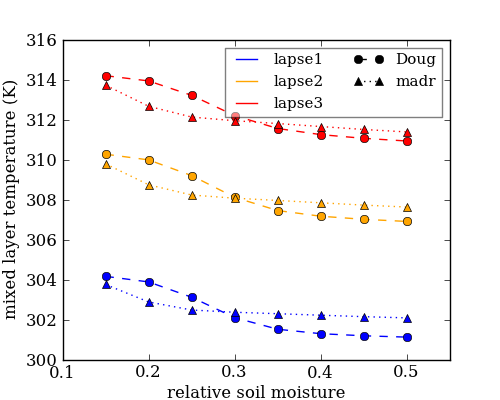
\includegraphics[width=\textwidth]{ch2-BL/figures/all_afternoon_T.png}
\caption{}
\end{subfigure}
\begin{subfigure}{0.5\textwidth}
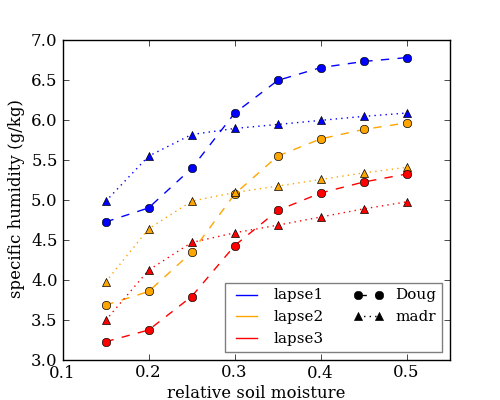
\includegraphics[width=\textwidth]{ch2-BL/figures/all_afternoon_Q.png}
\caption{}
\end{subfigure}
\caption{}
\label{fig:BL_345changes}
\end{figure}

%\clearpage

For both the Pacific madrone forest and the Douglas fir forest, drier soil (decreasing $\theta_{rel}$) leads to a warmer and drier boundary layer (increasing $T_a$ and decreasing $Q$).  However, in the Douglas fir case, the increase in $T_a$ and decrease in $Q$ begin when the soil is wetter ($\theta_{rel} \le 0.3$; Figures \ref{fig:BL_1DdiurnalTa} and \ref{fig:BL_1DdiurnalQ}, left columns), while in the Pacific madrone case, the increase in $T_a$ and decrease in $Q$ begin only when soil is drier ($\theta_{rel} \le 0.2$; Figures \ref{fig:BL_1DdiurnalTa} and \ref{fig:BL_1DdiurnalQ}, right columns).  

The differences between the species cases are largest in the afternoon; Figure \ref{fig:BL_345changes} shows $T_a$ and $Q$ at 3:45 pm for the Douglas fir and Pacific madrone cases, as a function of $\theta_{rel}$ and free troposphere conditions.  The differences between the Douglas fir and Pacific madrone cases for both $T_a$ and $Q$ are largest at $\theta_{rel}$ values around 0.2, with the Douglas fir case hotter by 1-1.5 $^\circ$C and drier by $\sim$0.7 g/kg.  A $\theta_{rel}$ value of 0.2-0.25 is typical for the mid- to late-dry-season at the ACRR [REF MET T SERIES FIG]. Interestingly, at $\theta_{rel}$ values higher than about 0.35, the Douglas fir case is actually cooler and moister; such $\theta_{rel}$ values are typical for the late spring and early summer at the ACRR [REF MET T SERIES FIG].

\begin{figure}[here]
\begin{subfigure}{0.5\textwidth}
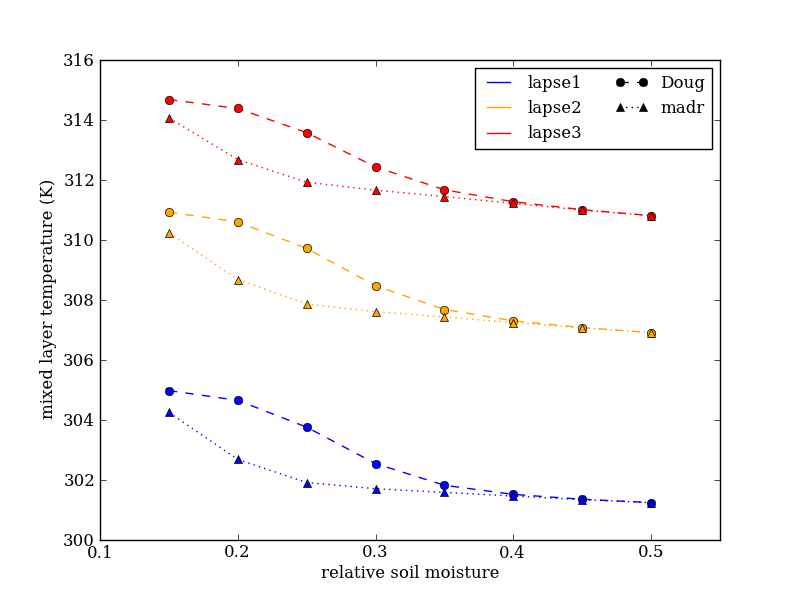
\includegraphics[width=\textwidth]{ch2-BL/figures/theta_afternoon_T.png}
\caption{}
\end{subfigure}
\begin{subfigure}{0.5\textwidth}
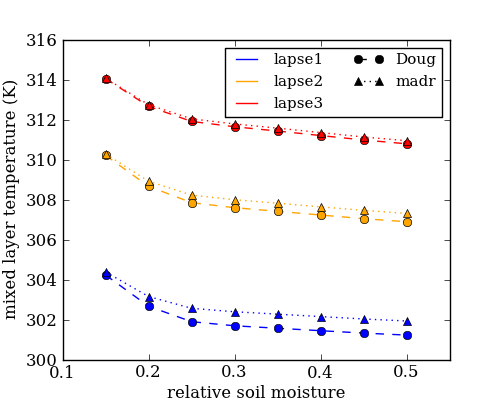
\includegraphics[width=\textwidth]{ch2-BL/figures/VPD_afternoon_T.png}
\caption{}
\end{subfigure}
\caption{}
\label{fig:BL_testVPDtheta}
\end{figure}

The temperature and humidity differences at $\theta_{rel} \le 0.3$ are due largely to Douglas firs' greater stomatal closure with dry soil.  Model tests holding the $VPD$ parameters constant at the Douglas fir values but varying the $\theta$ parameters give a Douglas fir - Pacific madrone temperature difference of 1.5-2$^\circ$C at $\theta_{rel} = 0.2$ (Figure \ref{fig:BL_testVPDtheta}(a)), while tests holding the $\theta$ parameters constant at the Pacific madrone values but varying the $VPD$ parameters give a temperature difference of \textless 0.5$^\circ$C at $\theta_{rel} = 0.2$ (Figure \ref{fig:BL_testVPDtheta}(b)).  Thus, in dry soil, the Douglas fir $VPD$ response does little to moderate the temperature differences caused by Douglas fir stomatal closure at low $\theta_{rel}$.  However, in wet soils ($\theta_{rel}$ \textless $0.3$), and particularly in cool free troposphere conditions, the greater Douglas fir stomatal conductance at low $VPD$ cools the boundary layer (Figure \ref{fig:BL_testVPDtheta}(b)), while soil moisture plays little role (Figure \ref{fig:BL_testVPDtheta}(a)).

%- fraction of moisture from land surface vs. from free troposphere, for different soil moisture / lapse rate / species conditions

\subsection{Regional climate model}

\begin{figure}[here]
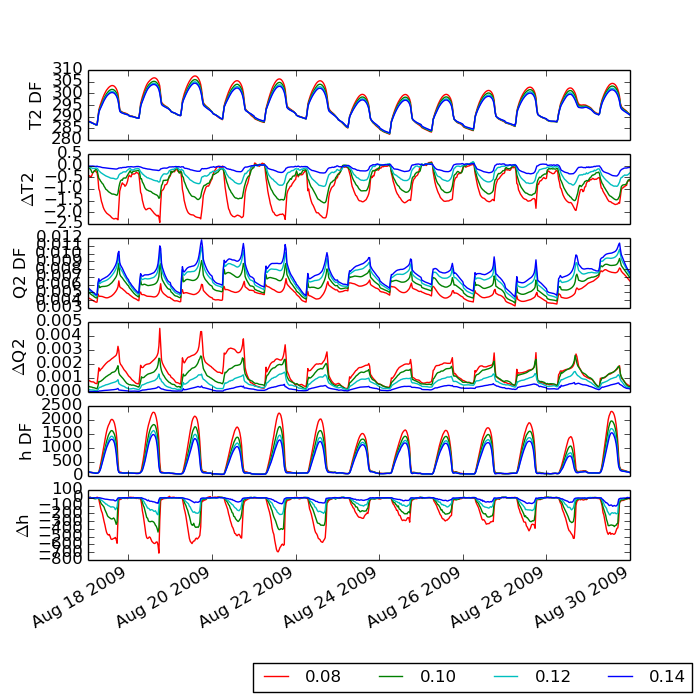
\includegraphics[width=0.85\textwidth]{ch2-BL/figures/T_Q_h_d02.png}
\caption{}
\label{fig:BL_WRFtseries}
\end{figure}

In the Douglas fir case, drier soils lead to a hotter, drier, and deeper boundary layer (panels 1, 3, and 5 of Figure XX).  For soil moisture $\le$ 0.12 m$^3$/m$^3$ ($\theta_{rel} \le XX$), the boundary layer over the madrone forest is cooler, moister, and shallower than that over the Douglas fir forest; the differences are negligible for soil moisture of 0.14 m$^3$/m$^3$ ($\theta_{rel} = XX$).  The differences between the species cases increase with drier soil: the greatest differences occur when soil moisture is 0.08 m$^3$/m$^3$, with 2 m air temperature in the madrone case cooler by 1.5-2.5$^\circ$C, 2 m humidity greater by 1-3 g/kg, and boundary layer depth shallower by 200-500 m, averaged over the test region (Figure XX, panels 2, 4, and 6).  The 2 m temperature and humidity are not equivalent to the mixed layer temperature in the 1-D model, because 2 m is well within the surface layer and is not in the mixed layer.  However, we show the 2 m conditions because they are relevant for ecosystems and people.

\begin{figure}[here]
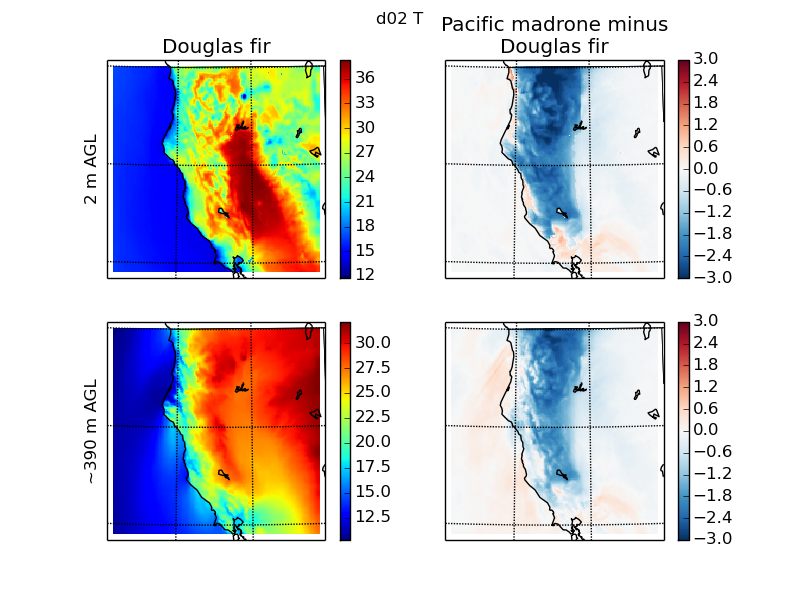
\includegraphics[width=1\textwidth]{ch2-BL/figures/T_d02_s0pt08.png}
\caption{}
\label{fig:BL_WRFmapT}
\end{figure}

\begin{figure}[here]
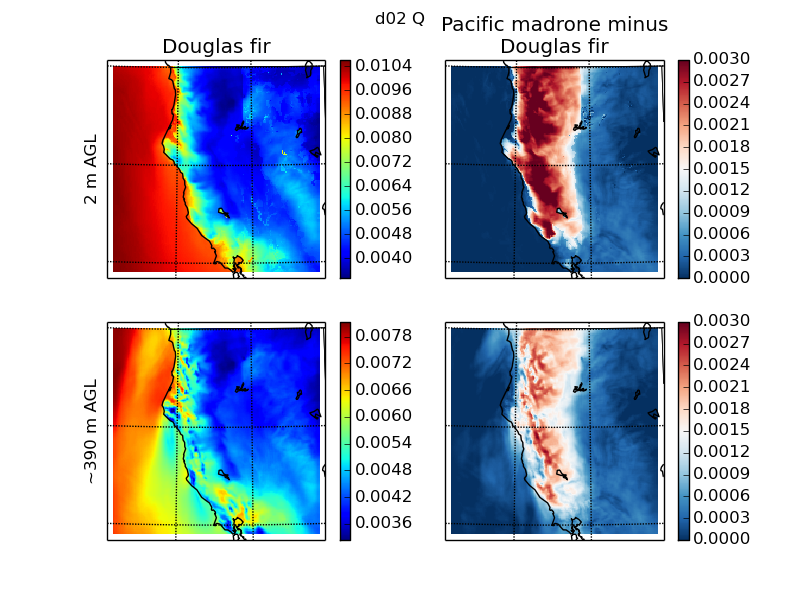
\includegraphics[width=1\textwidth]{ch2-BL/figures/Q_d02_s0pt08.png}
\caption{}
\label{fig:BL_WRFmapQ}
\end{figure}

\begin{figure}[here]
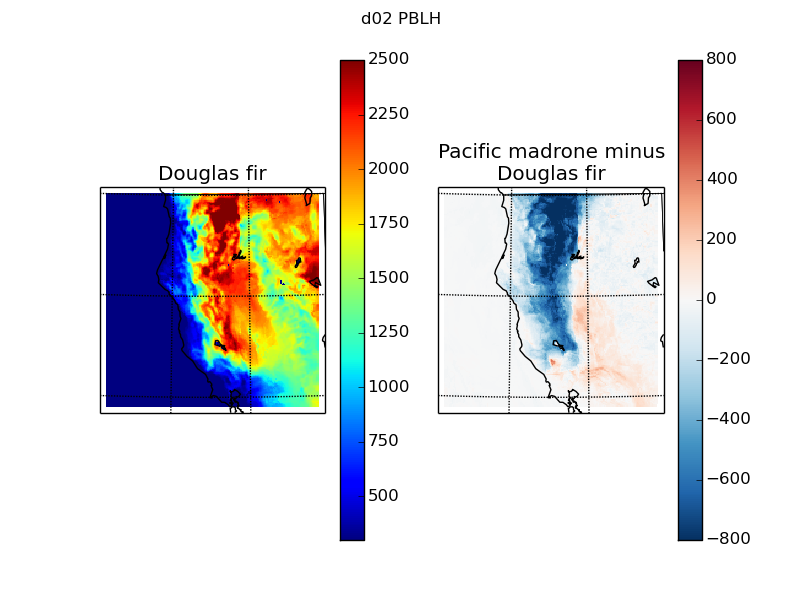
\includegraphics[width=1\textwidth]{ch2-BL/figures/PBLH_d02_s0pt08.png}
\caption{}
\label{fig:BL_WRFmapPBLH}
\end{figure}

The differences in temperature and humidity persist from 2 m above ground (Figures XX and XX, top rows) through to the mixed layer at $\sim$390 m above ground (Figures XX and XX, bottom rows). The species differences are smaller at 390 m than at 2 m above ground: the madrone case is cooler than the Douglas fir case by up to $\sim$2.5$^\circ$C at 2 m above ground and by up to $\sim$1.5$^\circ$C at 390 m above ground; humidity in the madrone case is greater than in the Douglas fir case by 2-3 g/kg at 2 m above ground and by 1.5-2.5 g/kg at 390 m above ground.

The changes in 390 m temperature and humidity and in boundary layer depth are greatest inland, where the convective boundary layer is fully developed.  The boundary layer in the control Douglas fir case is shallow near the coast but deepens inland (Figure XX, left panel).  In the coastal zone, it is likely that advection from the ocean is strong, and the boundary layer has not adjusted to the land surface.  The deeper boundary layer inland means that the air at 390 m above ground is part of the mixed layer that communicates rapidly with the surface; thus, the changes in temperature and humidity in the madrone case affect the air at 390 m above ground over inland but not coastal regions.


